% Options for packages loaded elsewhere
\PassOptionsToPackage{unicode}{hyperref}
\PassOptionsToPackage{hyphens}{url}
\PassOptionsToPackage{dvipsnames,svgnames*,x11names*}{xcolor}
%
\documentclass[
]{article}
\usepackage{lmodern}
\usepackage{setspace}
\usepackage{amssymb,amsmath}
\usepackage{ifxetex,ifluatex}
\ifnum 0\ifxetex 1\fi\ifluatex 1\fi=0 % if pdftex
  \usepackage[T1]{fontenc}
  \usepackage[utf8]{inputenc}
  \usepackage{textcomp} % provide euro and other symbols
\else % if luatex or xetex
  \usepackage{unicode-math}
  \defaultfontfeatures{Scale=MatchLowercase}
  \defaultfontfeatures[\rmfamily]{Ligatures=TeX,Scale=1}
\fi
% Use upquote if available, for straight quotes in verbatim environments
\IfFileExists{upquote.sty}{\usepackage{upquote}}{}
\IfFileExists{microtype.sty}{% use microtype if available
  \usepackage[]{microtype}
  \UseMicrotypeSet[protrusion]{basicmath} % disable protrusion for tt fonts
}{}
\makeatletter
\@ifundefined{KOMAClassName}{% if non-KOMA class
  \IfFileExists{parskip.sty}{%
    \usepackage{parskip}
  }{% else
    \setlength{\parindent}{0pt}
    \setlength{\parskip}{6pt plus 2pt minus 1pt}}
}{% if KOMA class
  \KOMAoptions{parskip=half}}
\makeatother
\usepackage{xcolor}
\IfFileExists{xurl.sty}{\usepackage{xurl}}{} % add URL line breaks if available
\IfFileExists{bookmark.sty}{\usepackage{bookmark}}{\usepackage{hyperref}}
\hypersetup{
  pdftitle={Measuring Perceptions and Preferences for Meritocracy},
  colorlinks=true,
  linkcolor=blue,
  filecolor=Maroon,
  citecolor=Blue,
  urlcolor=Blue,
  pdfcreator={LaTeX via pandoc}}
\urlstyle{same} % disable monospaced font for URLs
\usepackage[margin=0.78in]{geometry}
\usepackage{longtable,booktabs}
% Correct order of tables after \paragraph or \subparagraph
\usepackage{etoolbox}
\makeatletter
\patchcmd\longtable{\par}{\if@noskipsec\mbox{}\fi\par}{}{}
\makeatother
% Allow footnotes in longtable head/foot
\IfFileExists{footnotehyper.sty}{\usepackage{footnotehyper}}{\usepackage{footnote}}
\makesavenoteenv{longtable}
\usepackage{graphicx,grffile}
\makeatletter
\def\maxwidth{\ifdim\Gin@nat@width>\linewidth\linewidth\else\Gin@nat@width\fi}
\def\maxheight{\ifdim\Gin@nat@height>\textheight\textheight\else\Gin@nat@height\fi}
\makeatother
% Scale images if necessary, so that they will not overflow the page
% margins by default, and it is still possible to overwrite the defaults
% using explicit options in \includegraphics[width, height, ...]{}
\setkeys{Gin}{width=\maxwidth,height=\maxheight,keepaspectratio}
% Set default figure placement to htbp
\makeatletter
\def\fps@figure{htbp}
\makeatother
\setlength{\emergencystretch}{3em} % prevent overfull lines
\providecommand{\tightlist}{%
  \setlength{\itemsep}{0pt}\setlength{\parskip}{0pt}}
\setcounter{secnumdepth}{5}
\usepackage{caption}
\captionsetup[figure, table]{labelfont={bf},labelformat={default},labelsep=period}
\usepackage{graphicx}
\usepackage{float}
\usepackage{booktabs}
\usepackage{longtable}
\usepackage{array}
\usepackage{multirow}
\usepackage{wrapfig}
\usepackage{float}
\usepackage{colortbl}
\usepackage{pdflscape}
\usepackage{tabu}
\usepackage{threeparttable}

\title{Measuring Perceptions and Preferences for Meritocracy}
\author{}
\date{\vspace{-2.5em}}

\begin{document}
\maketitle

\setstretch{1.5}
\emph{Abstract}

Economic and social inequality have raised growing concerns and crises
across societies. One of social science concepts associated to the
maintenance of inequality is the belief in meritocracy, which would
legitimize economic differences based on effort and talent. Despite its
wide use, empirical research on meritocracy is something relatively
novel. A number of studies have relied mostly in secondary data to
operationalize meritocracy, with a large variation in the use and
interpretation of survey items. Starting from a review of studies that
measure meritocracy, this article identifies a series of drawbacks and
inconsistencies within and between studies regarding the
conceptualization and measurement of meritocracy. Based on this critical
analysis, we propose an items battery called ``Perceptions and
preferences for meritocracy scale'', which is tested with confirmatory
factor analysis with data from an online survey study (N=2,141). The
results support the proposed conceptual structure which not only
distinguishes between perceptions and preferences, but also between
meritocratic and non-meritocratic dimensions. The discussion highlights
the relevance of considering these different dimensions in order to
advance in the study of meritocracy.

\hypertarget{introducciuxf3n}{%
\section{Introducción}\label{introducciuxf3n}}

La desigualdad económica se ha vuelto un tema que genera creciente
preocupación y malestar alrededor del mundo. Esto se ha expresado en una
serie de protestas como la emblemática ``occupy wall street'' el año
2011, así como también en una serie de análisis críticos respecto del
desarrollo del capitalismo y sus consecuencias ({\textbf{???}}). En este
contexto, el estudio de las visiones, preferencias y percepciones
respecto de la desigualdad han adquirido relevancia en las ciencias
sociales, en temas como las preferencias redistributivas (Alesina and
Angeletos \protect\hyperlink{ref-alesina_Fairness_2005}{2005}; Dimick,
Rueda, and Stegmueller \protect\hyperlink{ref-dimick_Models_2018}{2018})
la legitimación de la desigualdad económica (Schröder
\protect\hyperlink{ref-schroder_Income_2017}{2017}) y el funcionamiento
de la meritocracia ({\textbf{???}}; {\textbf{???}}; {\textbf{???}}).

En general, la meritocracia se define como un sistema de distribución de
recursos y recompensas basados en el mérito individual, que en su
concepción original es una suma de talento y esfuerzo (Young
\protect\hyperlink{ref-young_rise_1962}{1962}). Esta concepción
tradicional de mérito pone en un lugar secundario la posible
interferencia de factores estructurales o no meritocráticos como la
herencia, los contactos personales, o la suerte (Breen and Goldthorpe
\protect\hyperlink{ref-breenClassInequalityMeritocracy1999}{1999};
Saunders \protect\hyperlink{ref-saundersMightBritainBe1995}{1995}; Yair
\protect\hyperlink{ref-yairMeritocracy2007}{2007}; Land
\protect\hyperlink{ref-landWeSatTable2006}{2006}; Young
\protect\hyperlink{ref-youngRiseMeritocracy1994}{1994}). Una serie de
estudios han realizado críticas a la realización de este estándar moral
de distribución, planteando que es una promesa incumplida dada la
influencia preponderante de otros elementos más allá del mérito en el
estatus individual ({\textbf{???}}; Arrow, Bowles, and Durlauf
\protect\hyperlink{ref-arrow_meritocracy_2000}{2000}; Goldthorpe
\protect\hyperlink{ref-goldthorpe_myth_2003}{2003}; Markovits
\protect\hyperlink{ref-markovits_Meritocracy_2019}{2019}). Por otro
lado, desde la psicología social y la sociología se han estudiado las
características y consecuencias de las creencias en la meritocracia, en
general basados en la hipótesis que mayor creencia en la meritocracia
lleva a una mayor legitimación de las desigualdades ({\textbf{???}};
{\textbf{???}}; {\textbf{???}}; Hadjar
\protect\hyperlink{ref-hadjar_meritokratie_2008}{2008}; Madeira et al.
\protect\hyperlink{ref-MadeiraPrimesConsequencesSystematic2019}{2019}).

Debido al rol que cumplen las creencias meritocráticas dentro del
pensamiento neoliberal ({\textbf{???}}), han surgido múltiples
investigaciones que evalúan la relación entre creencias meritocráticas y
diversos ámbitos sociales de la actualidad. Por ejemplo, se han
desarrollado estudios que vinculan la meritocracia al reforzamiento de
estereotipos socioeconómicos, de género y de etnias (Madeira et al.
\protect\hyperlink{ref-MadeiraPrimesConsequencesSystematic2019}{2019};
{\textbf{???}}; {\textbf{???}}), así como también líneas de
investigación que evalúan el efecto de las creencias meritocráticas en
el contexto educativo ({\textbf{???}}; {\textbf{???}}; {\textbf{???}}) y
en el contexto organizacional de las empresas ({\textbf{???}};
{\textbf{???}}).

Para poder dar cuenta de los niveles de creencia en la meritocracia los
estudios a la fecha generalmente han utilizado algunos indicadores de
encuestas ya existentes, y en el menor de los casos se han creado
instrumentos ad-hoc. Sin embargo, y como mostraremos más adelante, las
formas de medición de meritocracia varían extremadamente entre estudios.
Muchas veces fenómenos similares se asocian a indicadores distintos, y
también ocurre que fenómenos distintos son medidos con indicadores
similares, todo lo cual hace dificulta la comparabilidad entre estudios
y el poder avanzar en la comprensión y estudio de la meritocracia.

Basados en el análisis crítico de las formas de medición de meritocracia
a la fecha, el presente artículo propone un instrumento para medir y
relacionar dos aspectos claves en el estudio de la meritocracia:
percepciones y preferencias. Además, como un segundo eje de análisis
considera la generación de indicadores respecto de aspectos
meritocráticos y anti-meritocráticos, demostrando que no son los dos
polos de un mismo continuo como muchos estudios anteriores parecen
sugerir. La propuesta de medición además está orientada a generar un
instrumento lo más breve posible de manera que pueda ser utilizado en
encuestas de opinión pública y así ser asociado a otros fenómenos
sociales.

\hypertarget{la-mediciuxf3n-de-los-aspectos-subjetivos-de-la-meritocracia}{%
\section{La medición de los aspectos subjetivos de la
meritocracia}\label{la-mediciuxf3n-de-los-aspectos-subjetivos-de-la-meritocracia}}

A continuación se presenta una revisión de una serie de investigaciones
que se han abocado al estudio de la meritocracia y que para ello han
hecho una propuesta de medición. El primer eje de análisis tiene que ver
con el uso del concepto ``creencias'' para referir a distintos aspectos
subjetivos relacionados con meritocracia. El segundo eje tiene que ver
con el uso de indicadores sobre aspectos anti-meritocráticos como el
polo opuesto de los meritocráticos.

\hypertarget{the-black-box-of-meritocratic-beliefs}{%
\subsection{The black-box of meritocratic
beliefs}\label{the-black-box-of-meritocratic-beliefs}}

Several approaches to the empirical study of meritocracy based on public
opinion surveys make reference to the concept of \emph{beliefs}, but
behind this concept there are usually different meanings and
operationalizations. To illustrate this point in the following we will
start with the proposal from a recent paper by Mijs
(\protect\hyperlink{ref-mijs_paradox_2019}{2019}), which we will take as
a reference to discuss previous studies.

The meritocratic beliefs' definition of Mijs is the following: ``when I
discuss meritocracy beliefs, I am referring to citizens' belief in the
importance of hard work relative to structural factors.'' (Mijs
\protect\hyperlink{ref-mijs_paradox_2019}{2019}, pg.9). In the
operationalization, this is associated with the following indicator:
``how important you think it is for getting ahead in life: (a) hard
work'', scored in a 1 to 5 likert scale. There are several assumptions
behind this decision that are worth discussing:

\begin{enumerate}
\def\labelenumi{\alph{enumi}.}
\tightlist
\item
  \emph{Dimensionality}
\end{enumerate}

The item used by Mijs is part of an items' battery present in several
international surveys, usually called ``reasons to get ahead''. This
battery presents a series of indicators related to what people consider
important to get ahead in life: hard work, education, ambition, wealthy
family, right connections, religion, race and gender. Therefore, for
Mijs other aspects as education, that could be associated to talent, are
not meritocratic. As he points out: ``Hard work is arguably the most
meritocratic part of Michael Young's equation, `Merit = Intelligence +
Effort', for the simple fact that intelligence itself is conditioned by
a nonmeritocratic factor: who your parents happen to be'' (p.5).

In Mijs' proposal we can observe a couple of strong assumptions: effort
would not depend on parents influence, and talent is not meritocratic
(contrary to Michael Youngs original conceptualization). The problem of
whether talent is or not meritocratic is something that actually should
(and can) be tested, it cannot be simply ruled out particularly in
empirical research. This conceptual and measurement issue it is possible
to find in other studies that assume that effort is the main and only
aspect of meritocracy ({\textbf{???}}; {\textbf{???}}; {\textbf{???}};
{\textbf{???}}).

\emph{b. Beliefs}

The ``resons to get ahead'' battery refers to ``how important you think
it is'', considered by Mijs as a belief in meritocracy for the item
regarding effort. Nevertheless, another version of this same battery in
the survey asks about ``how important you think it \emph{should} be''.
Which one of both is a ``belief''? According to ({\textbf{???}}) :
``Perceptions refer to subjective estimates of existing inequality
(i.e.~thoughts about what is). Beliefs are here defined as normative
ideas about just inequality (i.e.~thoughts about what should
be)''(p.359). Therefore, the referred paper would be actually using the
term beliefs referring to perceptions. The same occurs in Reynolds and
Xian (\protect\hyperlink{ref-reynolds_perceptions_2014}{2014}), who
explicitly use the term beliefs to talk about perceptions, whereas other
authors use different terms as attitudes (Kunovich and Slomczynski
(\protect\hyperlink{ref-kunovich_systems_2007}{2007})). The first
attempt to shed light on this confusion was made by Duru-Bellat and
Tenret (\protect\hyperlink{ref-duru-bellat_whos_2012}{2012}), who used
the item ``how important should the number of years spent in education
and training be in deciding how much money people ought to earn?'' for
``desired'' meritocracy (beliefs), whereas for ``perceived'' meritocracy
they use two items: ``Would you say that in your country, people are
rewarded for their efforts?'' and ``\ldots{} people are rewarded for
their skills?''.

Is the belief in meritocracy a perception or a desire/preference? In
order to expand the analitical conceptual framework, we believe that
both dimensions should be included in the analysis, as proposed by
Duru-Bellat and Tenret
(\protect\hyperlink{ref-duru-bellat_whos_2012}{2012}). This opens up
possibilities of analyzing whether perceptions and preferences are
actually the same (i.e.~correlation close to 1) or they are different
aspects of the same phenomenon. As Son Hing et al.
(\protect\hyperlink{ref-son_hing_merit_2011-1}{2011}) have pointed out,
``People can believe that outcomes ought to be distributed on the basis
of merit and yet vary in their perceptions of whether this is how
society currently operates'' (p.~435). In other words, normative beliefs
should be interpreted in the context of perception: a large normative
belief in meritocracy certainly means something totally different for
someone perceiving high meritocracy than for someone perceiving low
meritocracy. In order to avoid the confusion generated by the term
``belief'', we propose the terms meritocratic preferences and
meritocratic perceptions, as they better reflect the two dimension under
scrutiny.

\emph{c.~Non-meritocratic aspects}

Mijs (\protect\hyperlink{ref-mijs_paradox_2019}{2019}) makes reference
to some non-meritocratic aspects as talent, which is ruled out of the
operationalization of meritocracy. A different approach was followed by
Kunovich and Slomczynski
(\protect\hyperlink{ref-kunovich_systems_2007}{2007}), who decide to
include some non-meritocratic elements. Using the items' battery listing
a number of reasons about ``How important should be in deciding
pay\ldots{}'' (as Duru-Bellat and Tenret
(\protect\hyperlink{ref-duru-bellat_whos_2012}{2012}) for desired
meritocracy), he decided that reasons as education and responsibility
are meritocratic and pointed 1 if considered essential, whereas reasons
such as having a family and children were pointed 1 if they were
considered ``not important at all'' (i.e.~reverse coded). A similar
approach was taken by Newman, Johnston, and Lown
(\protect\hyperlink{ref-newman_false_2015}{2015}), reverse-coding
non-meritocratic items, similarly to what occurs with the ``Preference
for the Merit Principle Scale'' (Davey et al.
\protect\hyperlink{ref-davey_preference_1999}{1999}).

The assumption that meritocratic and non-meritocratic elements are the
poles of the same continuum was analyzed by Reynolds and Xian
(\protect\hyperlink{ref-reynolds_perceptions_2014}{2014}) using the same
``get ahead'' perceptions' battery items. They consider education,
ambition and hard work as meritocratic and other reasons such as wealthy
family and right connections and non-mertitocratic. Nevertheless,
despite making this distinction the author ends up subtracting one
dimension from the other, assuming that they are two poles of the same
continuum as Kunovich and Slomczynski
(\protect\hyperlink{ref-kunovich_systems_2007}{2007}) did. Still, taking
into account this research perspective, we suggest that non-meritocratic
aspects should be part of a meritocratic measurement but taken
independently and not adding or subtracting from meritocratic ones
unless it is empirically proved that they belong to the same conceptual
dimension.

\emph{d.~Accounting for measurement error}

Finally, most of the studies in meritocracy so far have not incorporated
the issue of measurement error ({\textbf{???}}), using single indicators
and/or simple average indexes for measuring meritocracy. Such strategy
assumes that the construct is measured perfectly by the indicators
chosen, going as far as proposing that "\ldots{} In choosing this
strategy of index construction, we argue that \emph{support for
meritocracy is not a latent variable} (Kunovich and Slomczynski
\protect\hyperlink{ref-kunovich_systems_2007}{2007}, 653--54). Some
advances were done by Reynolds and Xian
(\protect\hyperlink{ref-reynolds_perceptions_2014}{2014}) by doing a
principal component analysis of meritocratic and non-meritocratic
dimensions, but somewhat contradictorily they end up in a sum index
despite proving multidimensionality.

\hypertarget{an-instrument-proposal}{%
\subsection{An instrument proposal}\label{an-instrument-proposal}}

Based on the previous limitations and confussions in the measurement of
meritocracy presented in the previous section, in this paper we propose
and test an instrument with the following characteristics:

\begin{itemize}
\item
  Multidimensional, incorporating previous distinctions between
  preferences and perceptions as well as between meritocratic and
  non-meritocratic aspects.
\item
  Multiple indicators for each dimension, in order to account for
  measurement error in a confirmatory factor analysis context.
\item
  Based on previous indicators as far as possible, for the sake of
  comparability between studies
\item
  Brief, as to be used in a regular survey. In this point it differs for
  instance from the proposal of the ``Preference for the Merit Principle
  Scale'' (Davey et al.
  \protect\hyperlink{ref-davey_preference_1999}{1999}), as they use 15
  items just for one dimension (besides the problem of reverse-coding
  non-meritocratic items).
\end{itemize}

The proposed measurement framework is depicted in Figure 1:

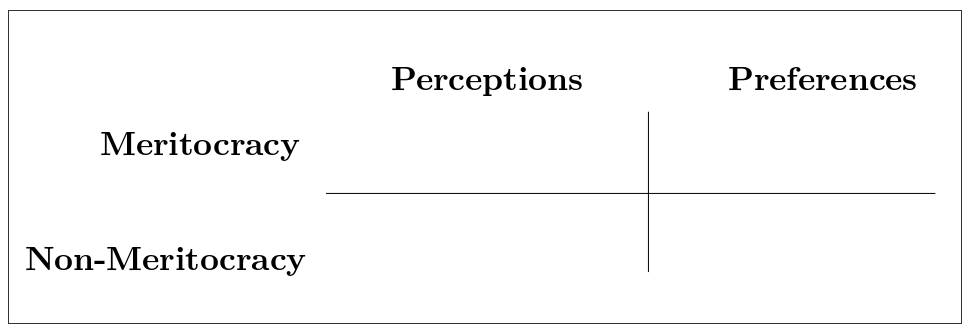
\includegraphics[width=0.6\textwidth,height=\textheight]{../input/images/generalf.png}

The columns Perceptions and Preferences represent the distinction
between this two concepts, usually confused under the label ``beliefs''.
Perceptions refers to the extent to which people see that meritocracy
functions or applies in their society, which in terms of measurement
relates to items such as ``I think hard work is important to get ahead
in society'', whereas preferences refer to normative expectations that
are usually linked to a ``should'' expression (e.g.~whether hard work
should be related to payment). The rows in the table of Figure 1
consider the distinction between meritocratic and non-meritocratic
dimensions (Reynolds and Xian
\protect\hyperlink{ref-reynolds_perceptions_2014}{2014}). This aspect
has been usually treated as different ends of a same continuum in part
of the previous research, an assumption that requieres empirical
scrutiny. These non-meritocratic elements usually refer to the use of
personal contacts or family advantages to get ahead in life.

Regarding the selection of indicators, most of them are taken or adapted
from previous studies for the sake of comparability. For meritocratic
indicators we use effort and talent as the main components of the
traditional concept of merit as defined by Young
(\protect\hyperlink{ref-young_rise_1962}{1962}), whereas for
non-meritocratic dimensions we use having rich parents and good
contacts. The description of the specific items is presented in the
methodology section.

The research hypotheses behind this conceptualization are the following:

\begin{itemize}
\item
  H1. The perception of meritocracy is a latent variable based on
  indicators of the importance attributed to talent and the effort to
  get ahead in life.
\item
  H2. The non-meritocratic perception is a latent variable that derives
  from two indicators related to the agreement with the statement that
  people with contacts and rich parents manage to get ahead.
\item
  H3. Meritocratic preferences are a latent variable based on a
  normative value of effort and talent.
\item
  H4. Non-meritocratic preferences are a latent variable based on the
  normative value of the use of personal contacts and having rich
  parents.
\end{itemize}

\hypertarget{methodology}{%
\section{Methodology}\label{methodology}}

\hypertarget{data-collection}{%
\subsection{Data collection}\label{data-collection}}

The data was obtained through an online questionnaire which was part of
a larger study on meritocracy and preferences developed in Chile in 2019
and funded by the national scientific agency FONDECYT. The questionnaire
was programmed in Qualtrics and the fieldwork was in charge of an
external online survey agency (\href{www.netquest.cl}{netquest.cl})
during December 2019 and January 2020. The sample was selected from a
non-probabilistic design in three large cities in Chile. The quota
method based on age, sex and educational level was used. Quotas were
generated based on the survey of the Public Studies Center (CEP, 2019),
which has a high prestige in the country and is also the counterpart
agency of ISSP (International Social Survey Programme) in Chile. A total
sample of 2,141 people was collected, excluding those who did not answer
the questions on the scale and those who did not accept informed
consent. As it usually occurs online samples, there were some
limitations in achieving the quotas for lower educational levels.

\hypertarget{instrument-design}{%
\subsection{Instrument design}\label{instrument-design}}

The proposed scale of perceptions and preferences about meritocracy
consists of 8 indicators that are grouped into the 4 dimensions referred
above: Perceptions (meritocratic/non-meritocratic) and preferences
(meritocratic/non-meritocratic). In order to achieve at least some
comparability with previous studies, the questions were adapted from the
items battery ``reasons to get ahead'' (ISSP/GSS), which are mostly used
for operationalizing meritocracy in previous empirical studies (Mijs
\protect\hyperlink{ref-mijs_paradox_2019}{2019}; Duru-Bellat and Tenret
\protect\hyperlink{ref-duru-bellat_whos_2012}{2012}; Reynolds and Xian
\protect\hyperlink{ref-reynolds_perceptions_2014}{2014}). The eight
items ordered according to dimensions are presented in Table 2. These 8
likert-type items have 5 response alternatives ranging from ``Completely
disagree''(1) to ``Completely agree'' (5).

\begin{table}[!h]

\caption{\label{tab:unnamed-chunk-6}Items according to dimension.}
\centering
\resizebox{\linewidth}{!}{
\fontsize{14}{16}\selectfont
\begin{tabu} to \linewidth {>{\raggedright\arraybackslash}p{1.5cm}>{\raggedright\arraybackslash}p{2 cm}>{\raggedright}X>{\raggedright}X}
\toprule
Dimension & Factor & Statement (english) & Statement (spanish)\\
\midrule
 &  & Those who try harder get greater rewards than those who work less. & Quienes más se esfuerzan logran obtener mayores recompensas que quienes se esfuerzan menos.\\
\cmidrule{3-4}
 & \multirow{-2}{2 cm}{\raggedright\arraybackslash Meritocratic} & Those who have more talent achieve greater rewards than those who have less talent. & Quienes poseen más talento logran obtener mayores recompensas que quienes poseen menos talento.\\
\cmidrule{2-4}
 &  & Those who have rich parents succeed. & Quienes tienen padres ricos logran salir adelante.\\
\cmidrule{3-4}
\multirow{-4}{1.5cm}{\raggedright\arraybackslash Perception} & \multirow{-2}{2 cm}{\raggedright\arraybackslash Non meritocratic} & Those who have good contacts succeed. & Quienes tienen buenos contactos logran salir adelante.\\
\cmidrule{1-4}
 &  & Those who try harder should get greater rewards than those who work less. & Quienes más se esfuerzan deberían obtener mayores recompensas que quienes se esfuerzan menos.\\
\cmidrule{3-4}
 & \multirow{-2}{2 cm}{\raggedright\arraybackslash Meritocratic} & Those who have more talent should get greater rewards than those who have less talent. & Quienes poseen más talento deberían obtener mayores recompensas que quienes poseen menos talento.\\
\cmidrule{2-4}
 &  & It's fine that those with rich parents get ahead. & Está bien que quienes tienen padres ricos salgan adelante.\\
\cmidrule{3-4}
\multirow{-4}{1.5cm}{\raggedright\arraybackslash Preference} & \multirow{-2}{2 cm}{\raggedright\arraybackslash Non meritocratic} & It's fine that those who have good contacts get ahead. & Está bien que quienes tienen buenos contactos salgan adelante.\\
\bottomrule
\end{tabu}}
\end{table}

\pagebreak

\hypertarget{administration-sets}{%
\subsection{Administration sets}\label{administration-sets}}

With the objective of evaluating the effect of the indicators ordering,
the respondents (\emph{n = 2141}) were randomly divided into three
different order versions as explained in \textbf{Figure 1}. The scale
was presented to the first group (\emph{n = 712}) in the order that
appears in Table 2. For the second group (\emph{n = 717}), the order of
the items was organized according to the topics of the items, e.g.~for
the topic of hard work the item about perception was followed by the
item about preference, and te same for the rest of the topics. Finally,
for the third group (\emph{n = 712}) the items were completely
randomized.

\begin{figure}
\centering
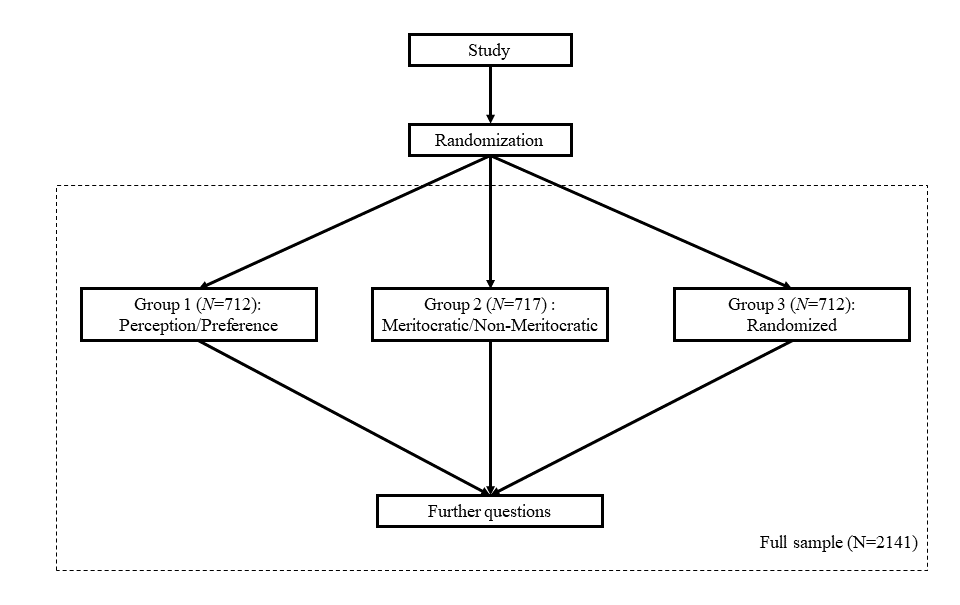
\includegraphics[width=0.8\textwidth,height=\textheight]{../input/images/app_mod.png}
\caption{Survey flow}
\end{figure}

\hypertarget{methods}{%
\subsection{Methods}\label{methods}}

For testing the scale's underlying constructs we estimate confirmatory
factor analysis models (CFA). The model estimates one factor for each
dimension, as represented in the following figure:

\begin{figure}
\centering
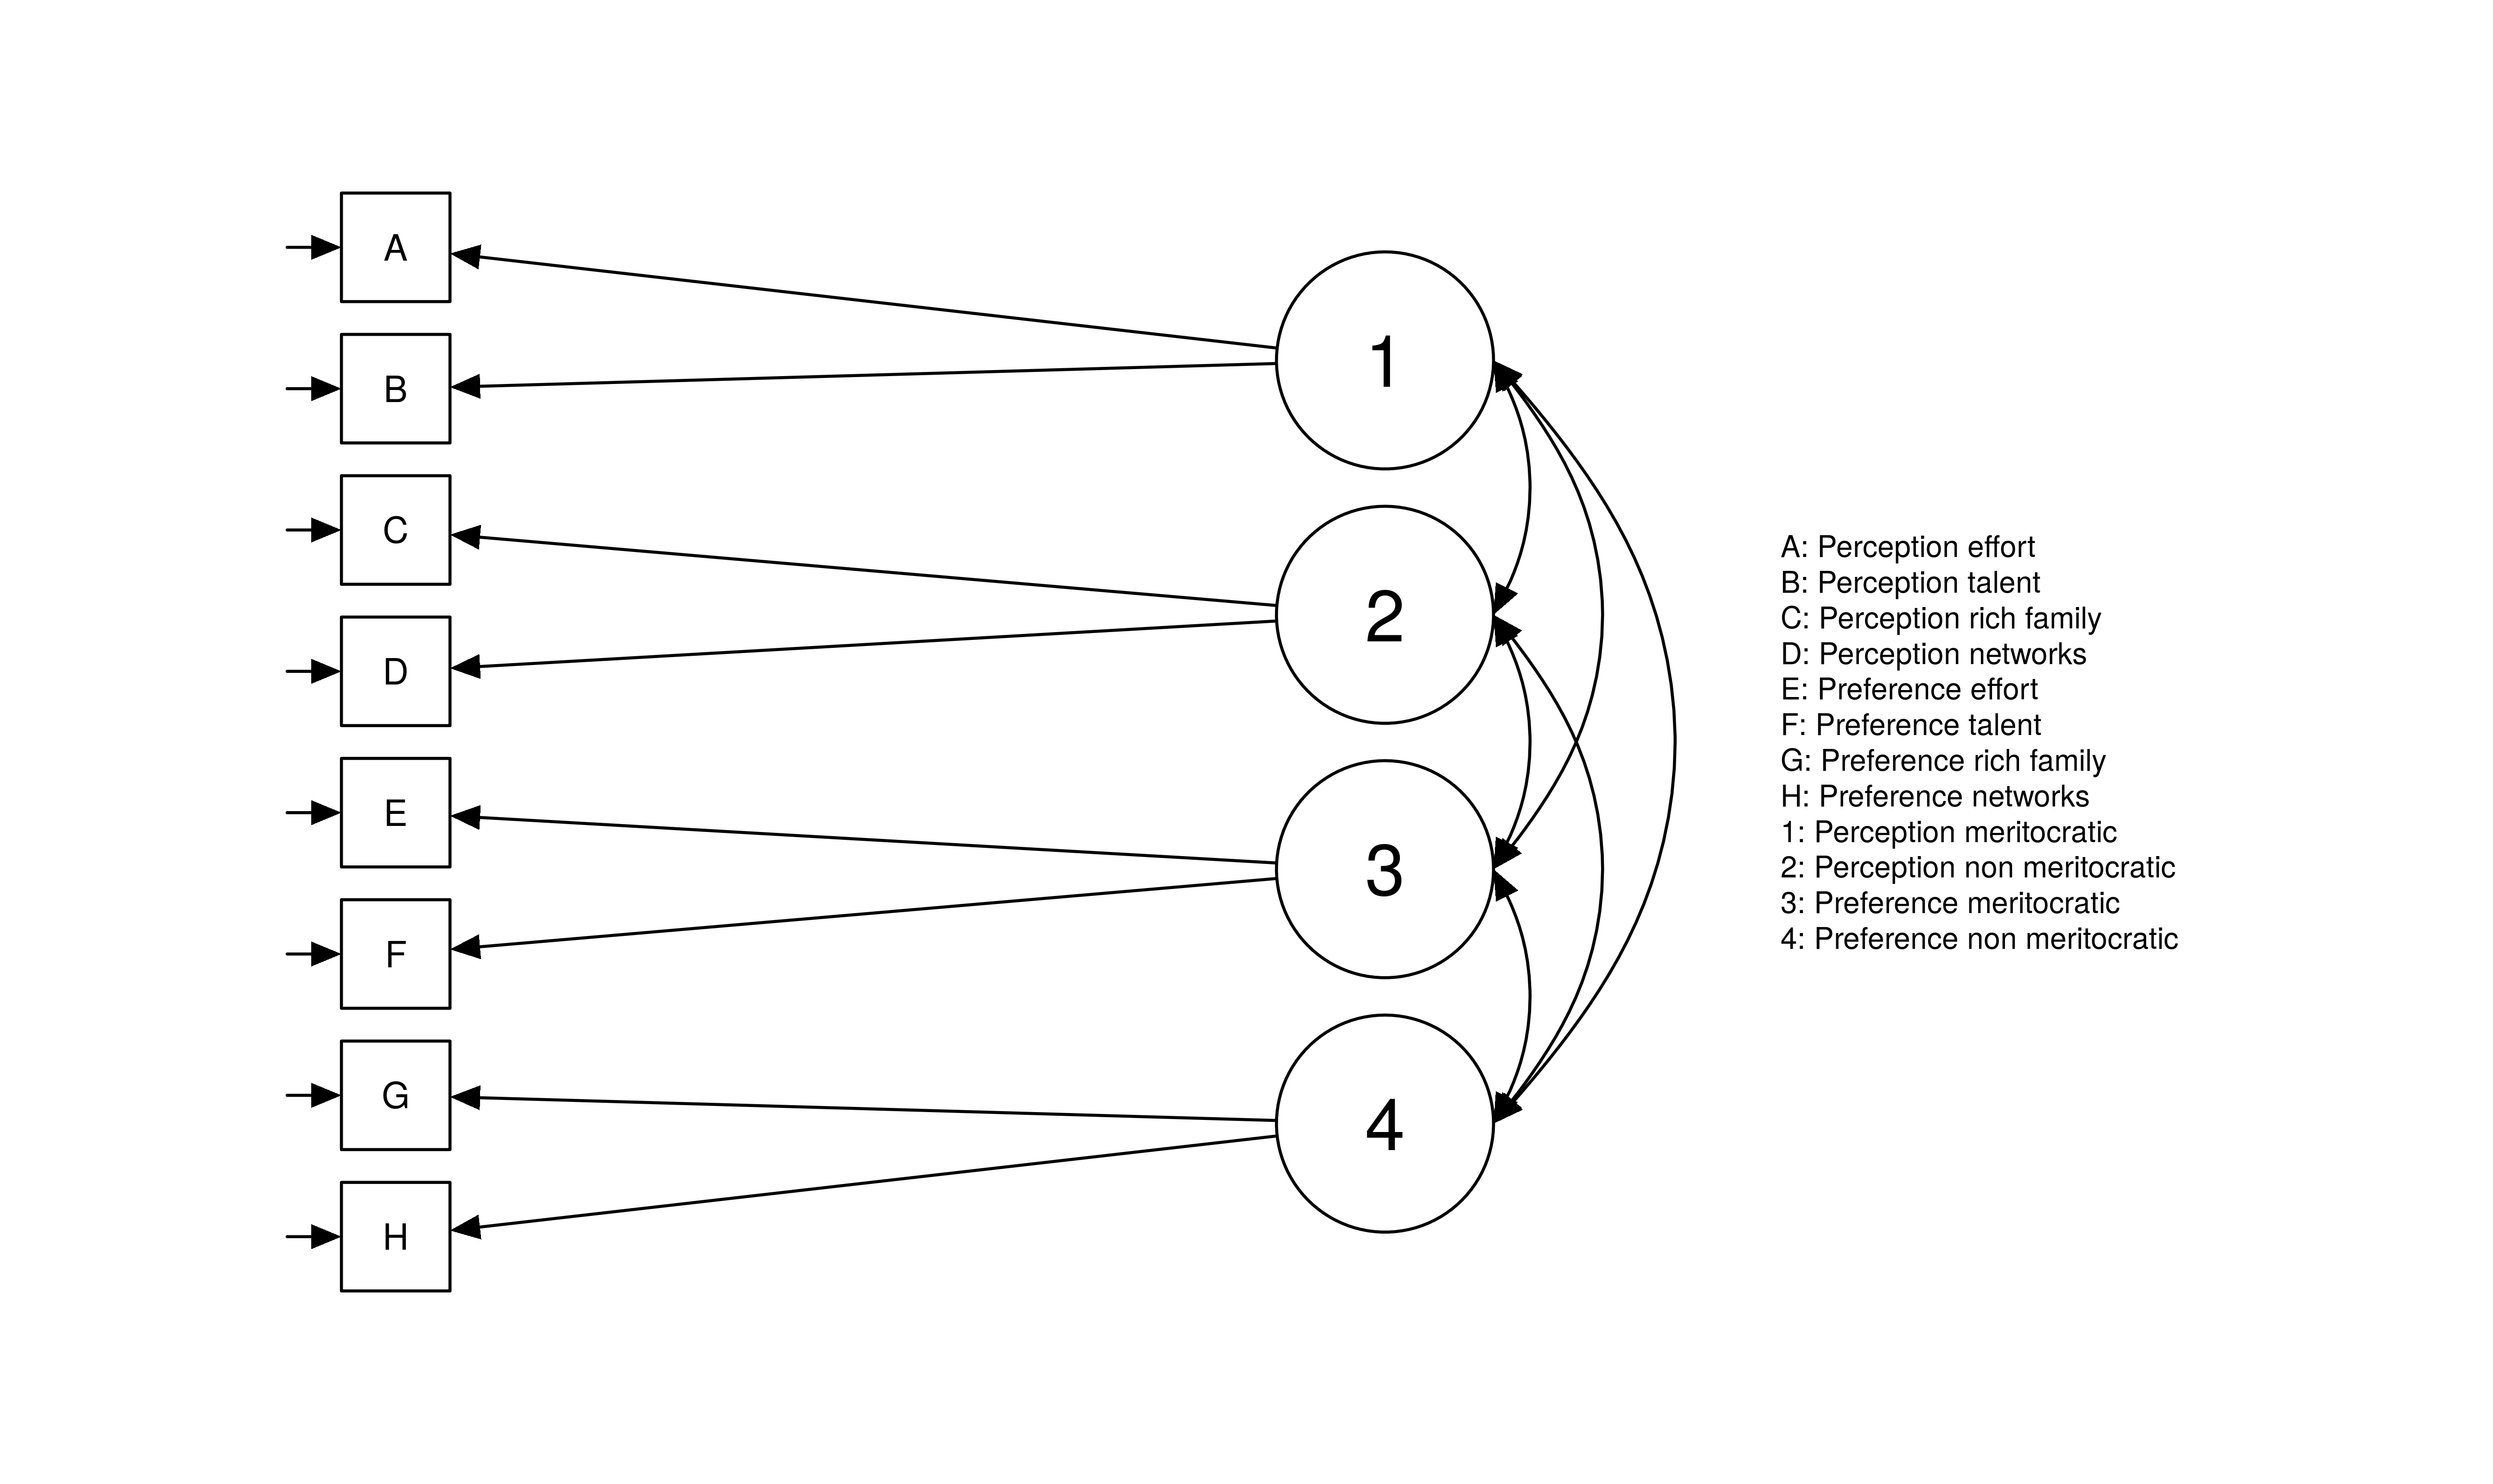
\includegraphics{../output/images/meas01.png}
\caption{Theorical model}
\end{figure}

CFA was conducted using the \texttt{lavaan} package (version 0.6-3;
Rosseel, 2020) with diagonally weighted least squares (DWLS) estimation
due to the items' ordinal level of measurement (Kline, 2016; Rosseel,
2020). As recommended by Brown (2008), we assessed model fit by jointly
considering the comparative fit index and Tucker-Lewis Index (CFI and
TLI; acceptable fit \textgreater{} 0.95), Root of the average squared
residual approximation (RMSEA; acceptable fit \textless{} 0.08),
Chi-square: (p-value; acceptable fit \textgreater{} 0.05, and Chi-square
ratio:\textgreater{} 3).

The study was pre-registered \ldots{} (link) ***

\hypertarget{results}{%
\section{Results}\label{results}}

\hypertarget{descriptive-analysis}{%
\subsection{Descriptive analysis}\label{descriptive-analysis}}

Como puede observarse en la tabla 3, los indicadores poseen valores que
van desde el 1 (totalmente en desacuerdo) al 5 (totalmente de acuerdo).
Se observan promedios desde 2.41 correspondiente a
preferencia-contactos, hasta 3.89 correspondiente a la
preferencia-esfuerzo. Ambos indicadores son coherentes con la adhesión
general a la meritocracia, privilegiando aspectos individuales como el
esfuerzo.

\begin{table}

\caption{\label{tab:unnamed-chunk-10}Descriptive statistics of the scale.}
\centering
\fontsize{9}{11}\selectfont
\begin{tabular}[t]{lllll}
\toprule
  & Mean & SD & Min & Max\\
\midrule
A.Perception Effort & 3.20 & 1.38 & 1 & 5\\
B.Perception Talent & 3.02 & 1.16 & 1 & 5\\
C.Perception rich parents & 3.66 & 1.36 & 1 & 5\\
D.Perception contacts & 3.79 & 1.24 & 1 & 5\\
E.Preferences Effort & 3.89 & 1.25 & 1 & 5\\
F.Preferences Talent & 3.24 & 1.19 & 1 & 5\\
G.Preferences rich parents & 2.69 & 1.18 & 1 & 5\\
H.Preferences contacts & 2.41 & 1.11 & 1 & 5\\
\bottomrule
\end{tabular}
\end{table}

El gráfico XX muestra \ldots{} A partir del gráfico se observa que en
general hay una mayor percepción de elementos no meritocráticos que
meritocráticos, mientras que en el caso de preferencias ocurre lo
opuesto. En cuanto a las preferencias, llama la atención el rol
preponderante del esfuerzo por sobre el talento.

\begin{figure}
\centering
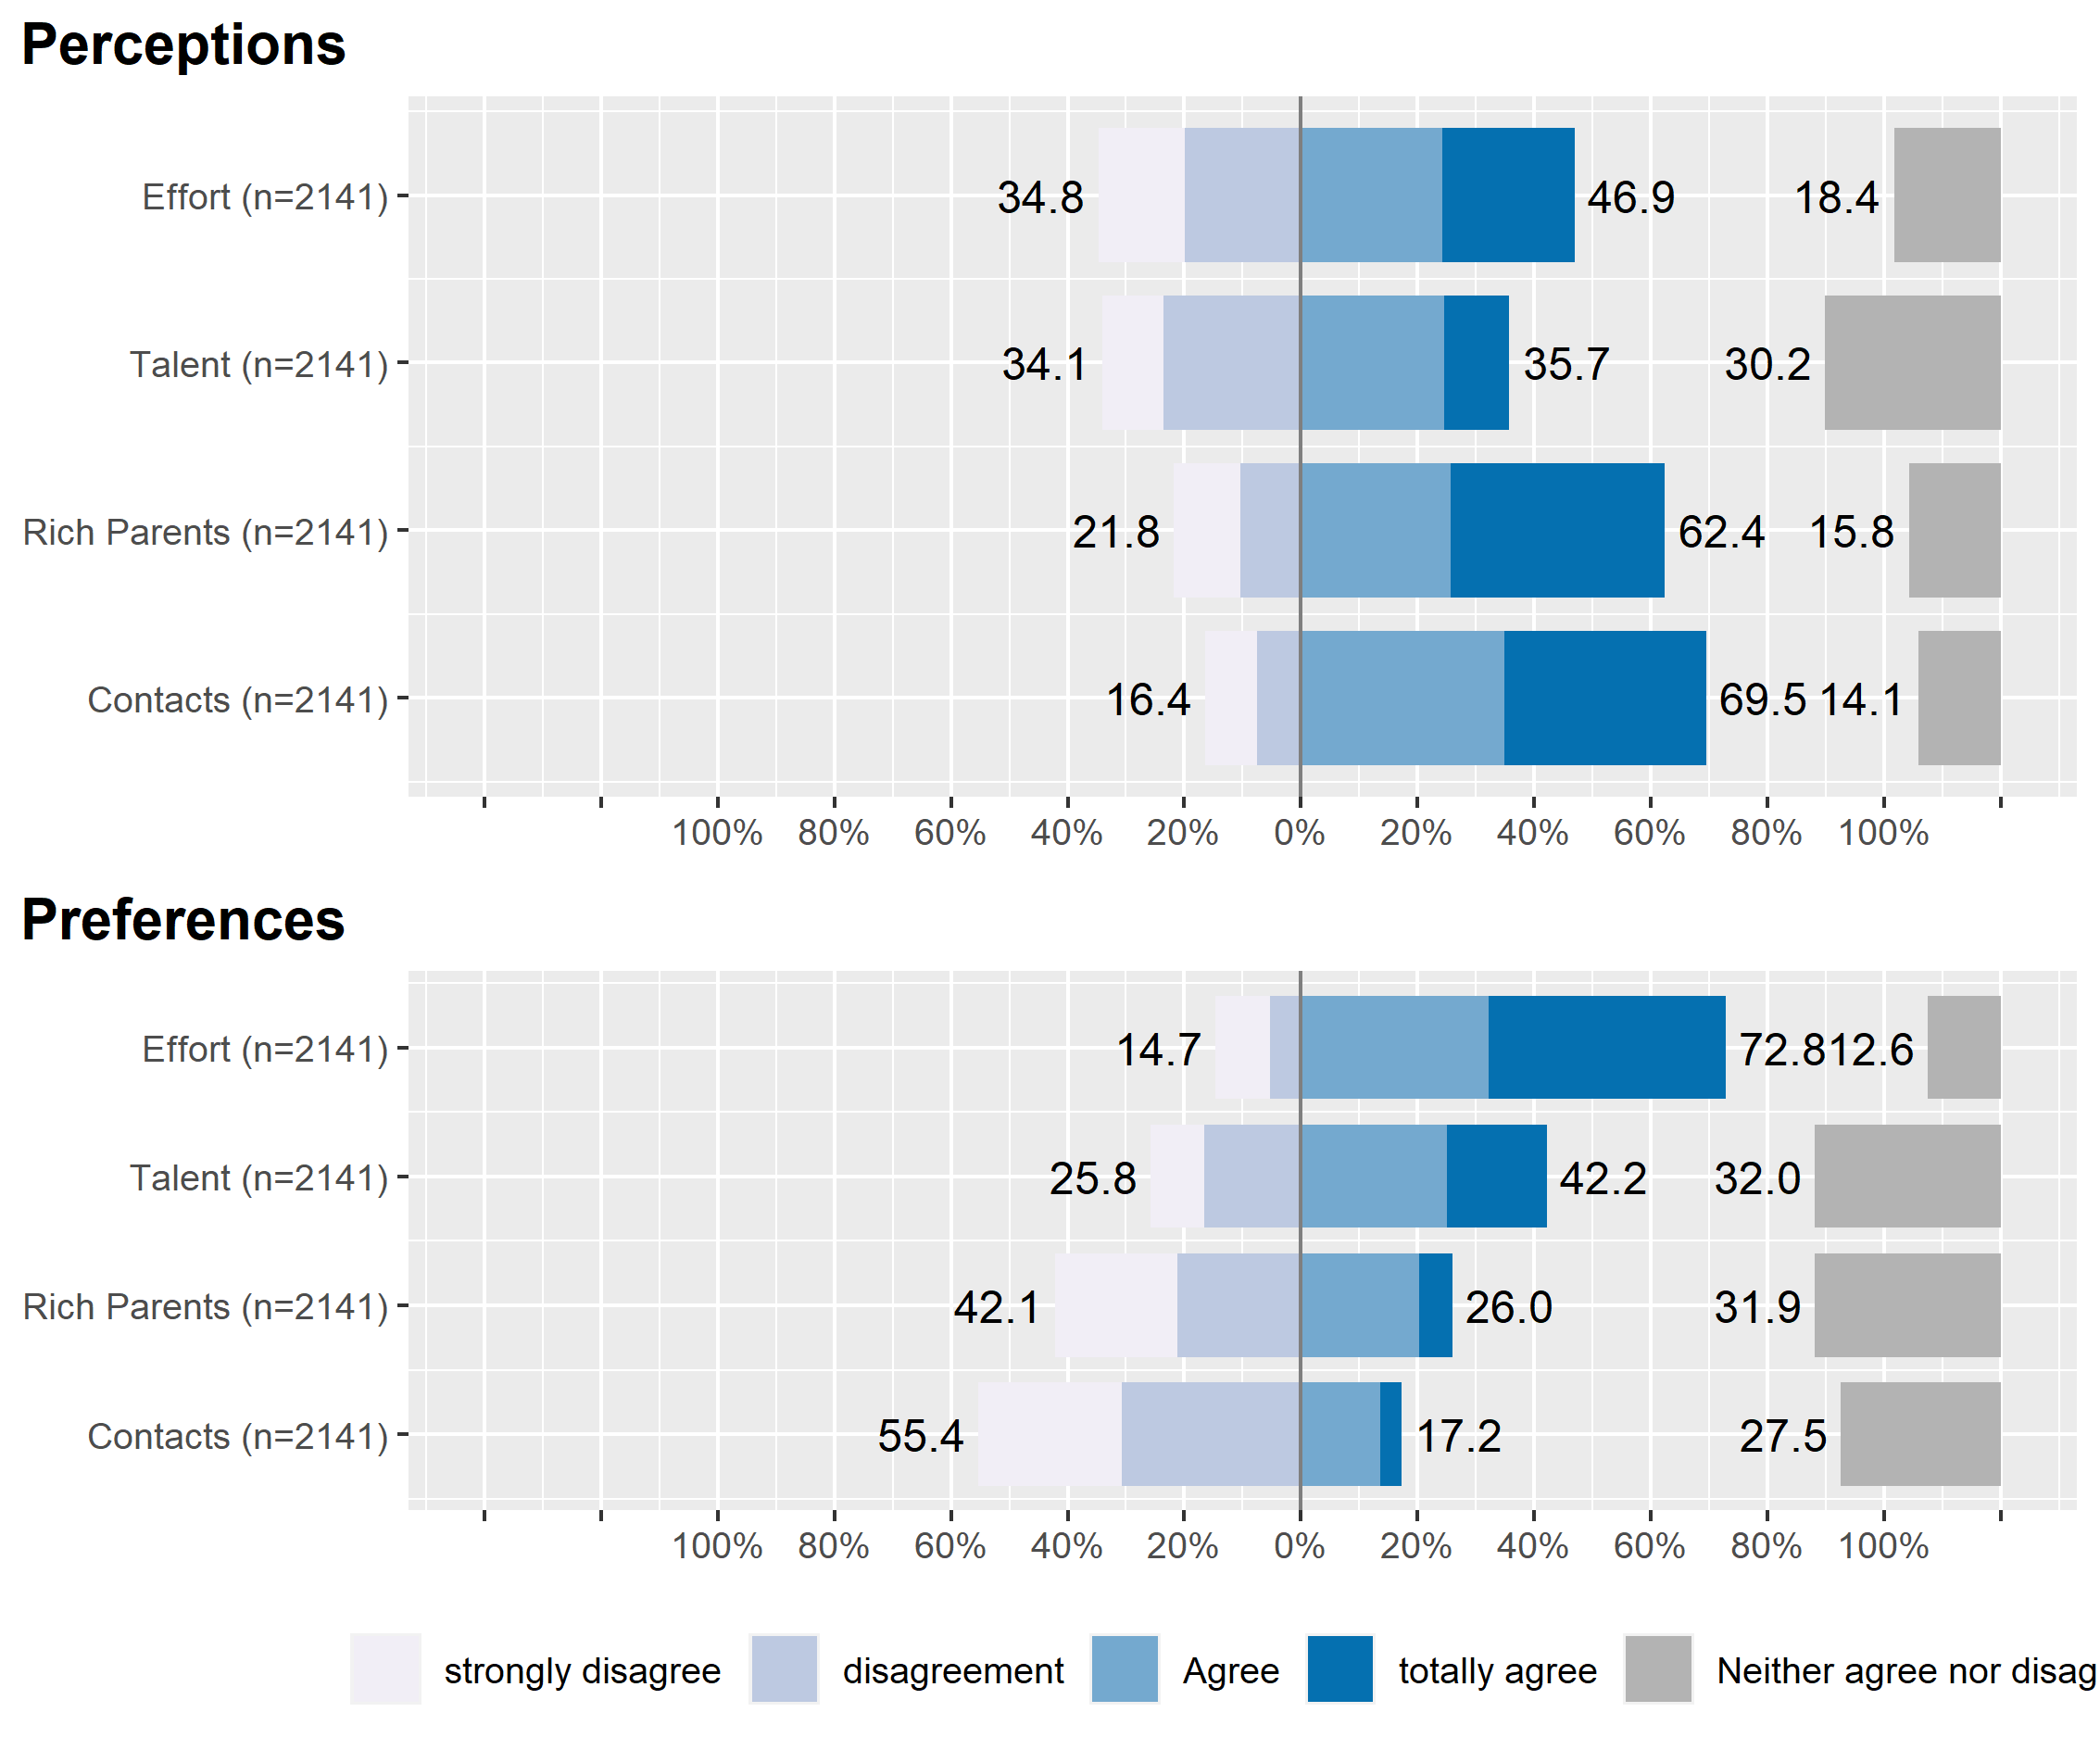
\includegraphics[width=11\textwidth,height=\textheight]{../output/images/plotlikert.png}
\caption{Descriptive plot}
\end{figure}

\pagebreak

El Grafico XX muestra \ldots. Se observan relaciones de moderada a alta
intensidad entre los indicadores que corresponden al mismo factor (por
ejemplo, percepción de meritocracia esfuerzo con talento r=0.56),
mientras que se observan correlaciones de baja intensidad entre el resto
de los cruces. Destacan además las relaciones entre las percepciones y
preferencias de tipo meritocráticas, lo que no ocurre con los
indicadores no meritocraticos.

\begin{figure}
\centering
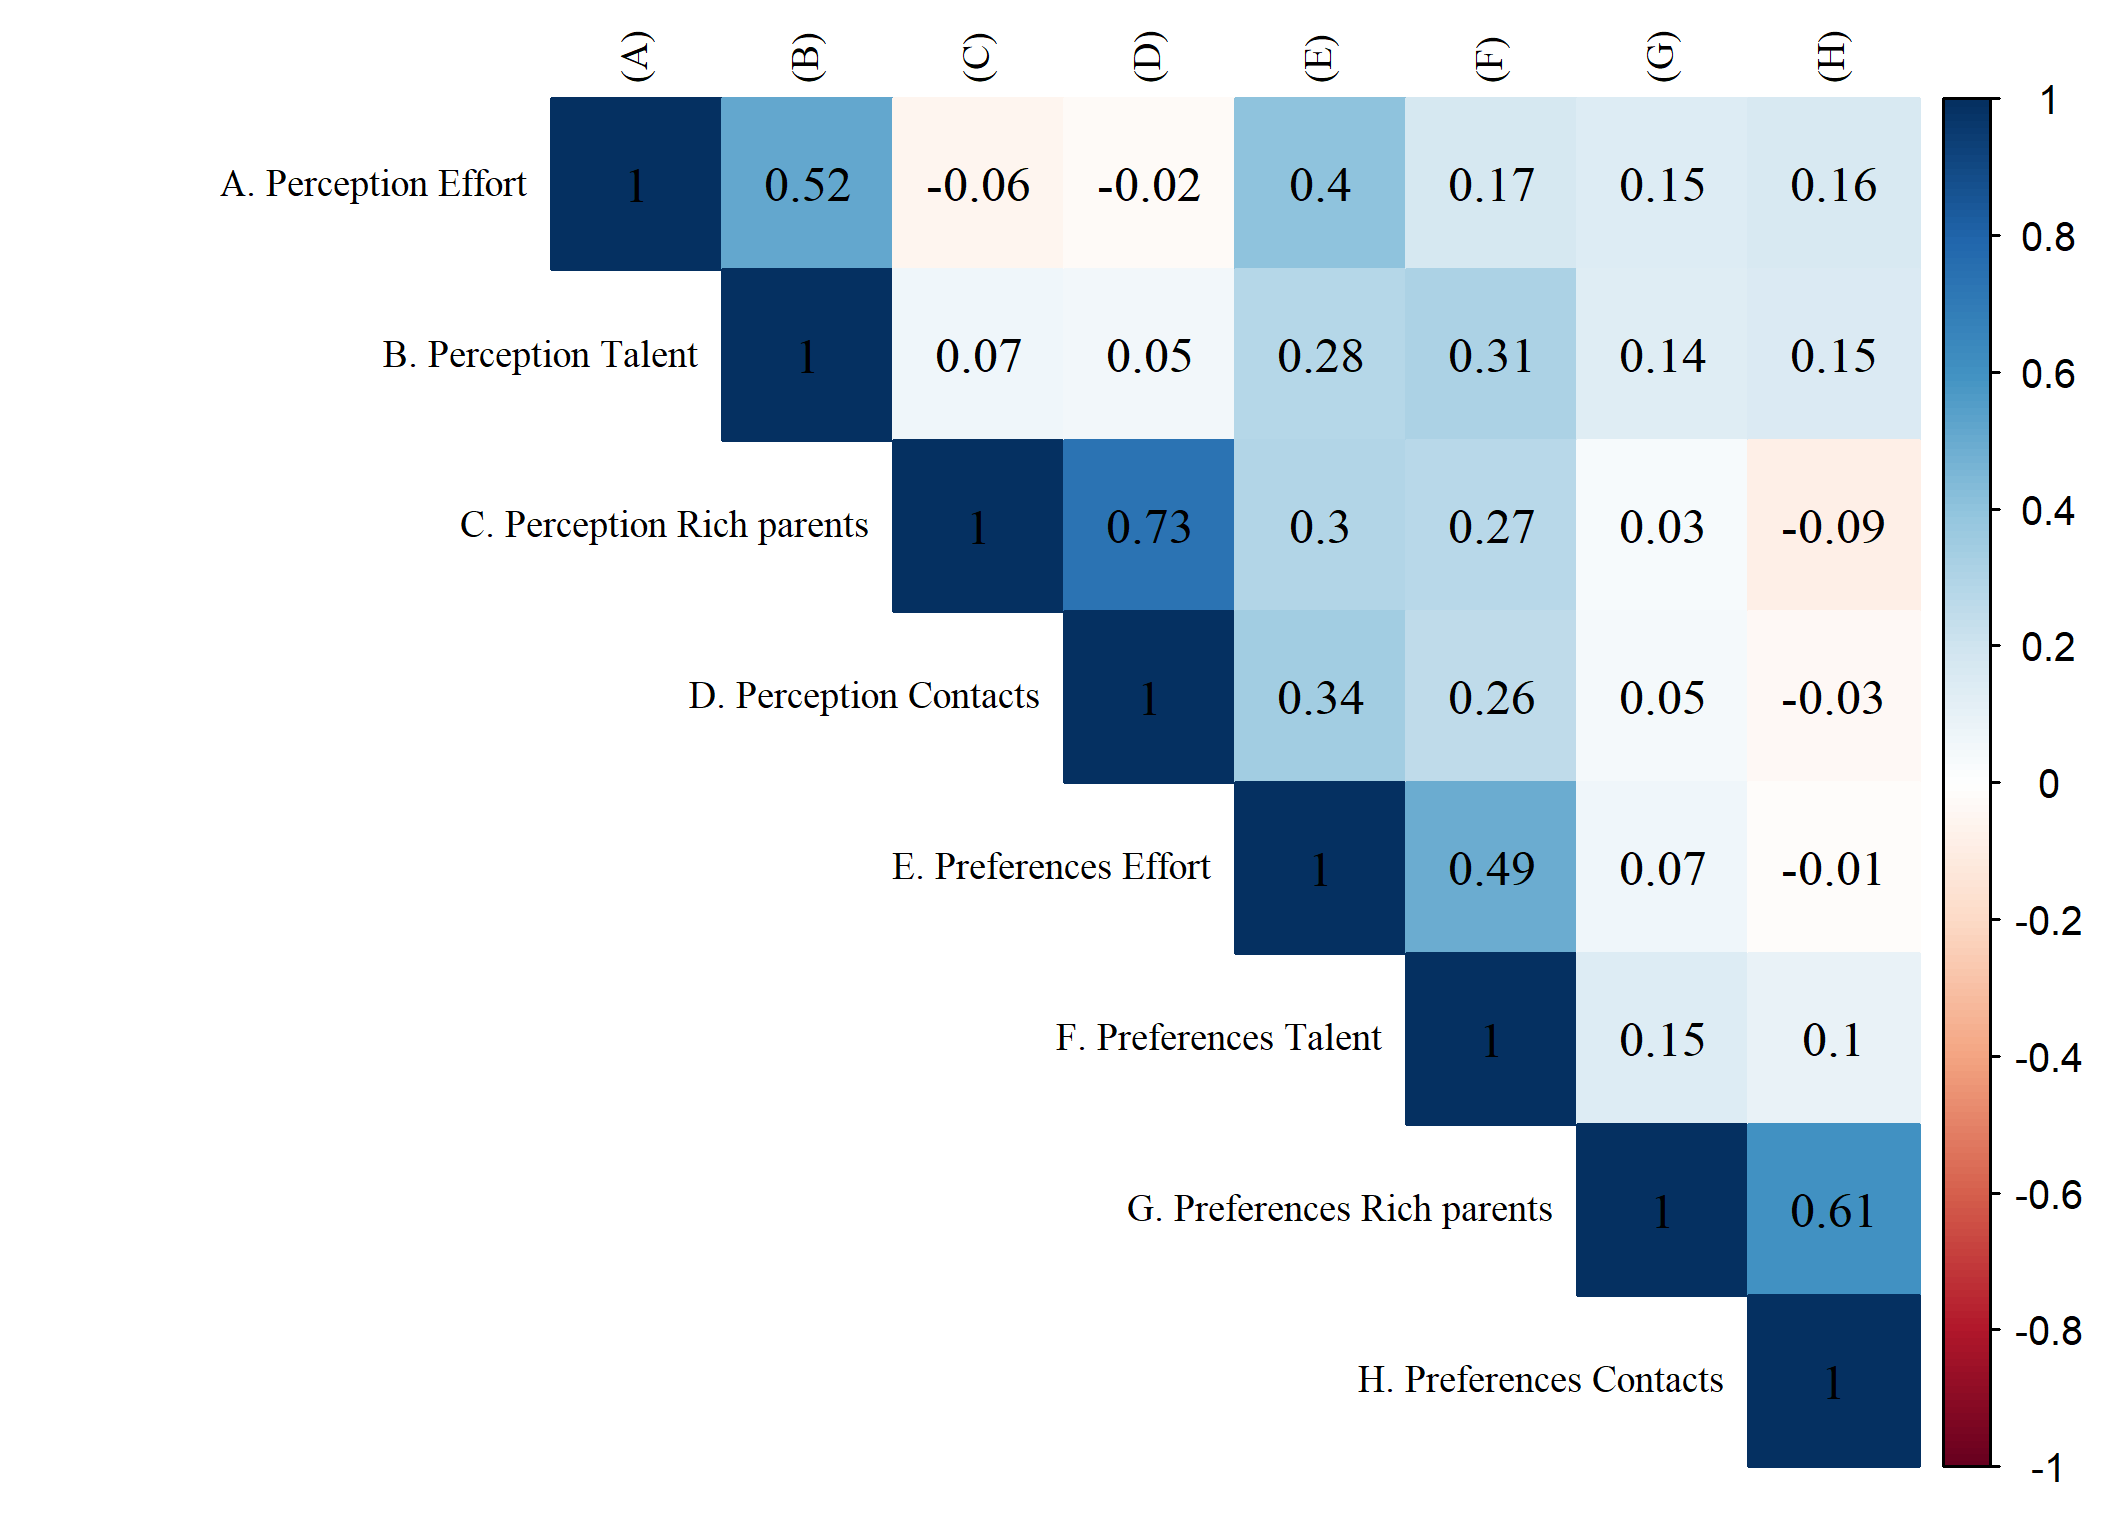
\includegraphics[width=0.9\textwidth,height=\textheight]{../output/images/corpoly.png}
\caption{polychoric correlation plot}
\end{figure}

En suma, los análisis descriptivos señalan una relativa adhesión a la
moral meritocratica, las cuales, a modo general, se expresan en una
mayor preferencia por criterios meritocraticos y una menor por no
meritocráticos. Igualmente, es observable una relativamente baja
percepción de meritocracia. Se observa además una relación coherente
entre los indicadores según lo propuesto en el modelo teórico en el
preregistro del estudio, es decir, los pares de items asociados a un
factor específico muestran correlaciones con un tamaño de efecto grande
(por ejemplo, preferencias meritocrácticas por los items asociados a
esfuerzo y a talento). En particular las asociaciones entre esfuerzo y
talento son relevantes, ya que desestiman previos supuestos sobre que el
talento no sería un criterio meritocrático (Mijs
\protect\hyperlink{ref-mijs_paradox_2019}{2019}), de otra manera la
correlación sería cero o negativa. Junto a ello, vemos que no existe una
correlacion negativa entre aspectos meritocráticos y no meritocráticos,
desestimando los supuestos de estudios previos que señalaban que estas
dimensiones serían los polos opuestos de un mismo continuo (Reynolds and
Xian \protect\hyperlink{ref-reynolds_perceptions_2014}{2014}).

\hypertarget{confirmatory-factor-analysis}{%
\subsection{Confirmatory Factor
Analysis}\label{confirmatory-factor-analysis}}

This section tests the item's battery and the corresponding conceptual
framework under test. For this, we first estimate a confirmatory factor
analysis model for the whole sample, and secondly we test the order
effects applying the same model to each of the three order versions.

\hypertarget{full-sample-cfa}{%
\subsubsection{Full sample CFA}\label{full-sample-cfa}}

Figure X shows the results of the estimation for the four-factor model:

Los modelos confirmatorios fueron estimados en primer lugar para cada
uno de los tres administration-sets. Los resultados se presentan en la
Tabla XX

\begin{table}[!h]

\caption{\label{tab:unnamed-chunk-14}Factor loads and model fit.}
\centering
\resizebox{\linewidth}{!}{
\fontsize{9}{11}\selectfont
\begin{threeparttable}
\begin{tabular}[t]{lcccccccccccc}
\toprule
\multicolumn{1}{c}{ } & \multicolumn{12}{c}{Factor loadings} \\
\cmidrule(l{3pt}r{3pt}){2-13}
\multicolumn{1}{c}{ } & \multicolumn{4}{c}{Version 1} & \multicolumn{4}{c}{Version 2} & \multicolumn{4}{c}{Version 3} \\
\cmidrule(l{3pt}r{3pt}){2-5} \cmidrule(l{3pt}r{3pt}){6-9} \cmidrule(l{3pt}r{3pt}){10-13}
Variables & 1 & 2 & 3 & 4 & 1 & 2 & 3 & 4 & 1 & 2 & 3 & 4\\
\midrule
Perception Effort & 0.69 &  &  &  & 0.76 &  &  &  & 0.70 &  &  & \\
Perception Talent & 0.81 &  &  &  & 0.72 &  &  &  & 0.65 &  &  & \\
Perception rich parents &  & 0.85 &  &  &  & 0.84 &  &  &  & 0.81 &  & \\
Perception contacts &  & 0.94 &  &  &  & 0.81 &  &  &  & 0.89 &  & \\
Preferences Effort &  &  & 0.85 &  &  &  & 0.82 &  &  &  & 0.66 & \\
Preferences Talent &  &  & 0.64 &  &  &  & 0.65 &  &  &  & 0.59 & \\
Preferences rich parents &  &  &  & 0.55 &  &  &  & 1.04 &  &  &  & 0.78\\
Preferences contacts &  &  &  & 1.26 &  &  &  & 0.52 &  &  &  & 0.77\\
\hline
\hspace{1em}$\chi^2\text{(df)}$ &  & 42.3(14) &  &  &  & 107.6(14) &  &  &  & 63.3(14) &  & \\
\hspace{1em}$\text{CFI}$ &  & 0.993 &  &  &  & 0.961 &  &  &  & 0.979 &  & \\
\hspace{1em}$\text{RMSEA}$ &  & 0.053 &  &  &  & 0.097 &  &  &  & 0.070 &  & \\
\hspace{1em}$N$ &  & 712 &  &  &  & 717 &  &  &  & 712 &  & \\
\bottomrule
\end{tabular}
\begin{tablenotes}
\item \textit{Note: } 
\item Standardised factor loadings using DWLS estimator ; CFI = Comparative fit index (scaled); RMSEA = Root mean square error of approximation (scaled)
\end{tablenotes}
\end{threeparttable}}
\end{table}

Como se puede observar en la Tabla XX, todos los modelos independiente
de los órdenes obtuvieron un ajuste adecuado. con CFI superiores a .95 y
RMSEA inferiores a .8, por contraparte ni un modelo logró un chi-square
no significativo, aunque tanto el modelo aleatorio como el primero
obtuvieron un adecuado chi-square ratio menor a 3. El primero de los
órdenes fue el que obtuvo mejor ajuste (CFI=0.998, TLI=
0.995,RMSEA=0.037, \(\chi2\)(df=14)=28,03, p = 0.014), seguido por el
orden aleatorio de los ítems (CFI=0.992, TLI=0.984,RMSEA=0.051,
\(\chi2\)(df=14)=39.09, p \textless{} 0.001). Por su parte, la escala
ordenada por temáticas parece generar un efecto framing en el cual la
relación entre las percepciones y las preferencias parecen
sobreestimadas, afectando de esta manera el ajuste (CFI=0.984,
TLI=0.968,RMSEA=.071, \(\chi2\)(df=14)=64.156, p \textless{} 0.001).

Si bien todas las pruebas obtuvieron indicadores relativamente
adecuados, las diferencias mencionadas entre los ajustes de los modelos
según orden son estadísticamente significativas, lo cual fue evaluado a
partir de un análisis de invarianza. Se concluye que entre los tres
órdenes no existe invarianza configuracional, es decir, no poseen la
misma dimensionalidad y por ello no ajustan igualmente al modelo teórico
({\textbf{???}}). Esto se debe al efecto producido por la aparición
conjunta de los ítems de un mismo factor en el orden 1, lo cual aumenta
el ajuste del modelo. Además, en el orden 2, al preguntarse seguidamente
por la percepción y la preferencia en torno al mismo indicador, aumentan
las relaciones cruzadas disminuyendo el ajuste del modelo. De modo
coherente, el modelo aleatorio presentó un ajuste intermedio entre el
orden 1 y el orden 2.

\pagebreak

\begin{longtable}[]{@{}cccc@{}}
\caption{Items according to dimension.}\tabularnewline
\toprule
& Contrast Model 1 Factor & theoretical model 4 Factors & Model with
M.I.\tabularnewline
\midrule
\endfirsthead
\toprule
& Contrast Model 1 Factor & theoretical model 4 Factors & Model with
M.I.\tabularnewline
\midrule
\endhead
\textbf{n} & 1769 & 1769 & 1769\tabularnewline
\textbf{CFI} & 0.595 & 0.988 & 0.994\tabularnewline
\textbf{TLI} & 0.433 & 0.976 & 0.985\tabularnewline
\textbf{RMSEA} & 0.226 & 0.047 & 0.036\tabularnewline
\textbf{\(\chi2\)} & 1830.839 & 68.661 & 40.250\tabularnewline
\textbf{p} & .000 & .000 & .000\tabularnewline
\textbf{\(\chi2\)/df} & 65.38 & 4.90 & 3.32\tabularnewline
\bottomrule
\end{longtable}

EL modelo teórico propuesto de cuatro factores ajustó, como se observa
en la tabla 4, mejor que el modelo de contraste de 1 factor. El modelo
teórico ajustó de manera relativamente adecuada, pues muestra
indicadores óptimos para CFI= 0.987, TLI = 0.975 y RMSEA=.041, aunque
posee indicadores deficientes para la prueba \(\chi2\)(df=14)=67.6,
p-value=.000. Para evaluar posibles mejoras de la escala, se analizaron
las relaciones propuestas por los índices de modificación. Estos indican
la existencia de dos cargas cruzadas no especificadas. Cuando se generó
un modelo siguiendo estas recomendaciones, hubo una mejora considerable
del modelo, aunque el nuevo modelo tampoco obtuvo un \(\chi2\) ratio
menor a 3 y obtuvo cargas factoriales muy bajas (\(\tau\))\textless{}
0.15, por lo tanto, siguiendo las recomendación de Brown (2006) de solo
aceptar las propuesta de los índices de modificación cuando se posee
teoria y evidencia sólida, se ha decidido no incorporar estos parámetros
al modelo.

\hypertarget{conclusiuxf3n}{%
\section{Conclusión}\label{conclusiuxf3n}}

Considerando la ventaja del orden, respecto aleatorio despeja la
posibilidad del efecto framing, es decir, de que el resultado del modelo
se deba al orden de las preguntas, se ha decidido seguir utilizando el
orden 3.

uso conjunto percepciones-preferencias

\pagebreak

\hypertarget{anexos}{%
\section{Anexos}\label{anexos}}

\begin{longtable}[]{@{}lcc@{}}
\caption{Representativeness of the sample.}\tabularnewline
\toprule
& Sample & CEP\tabularnewline
\midrule
\endfirsthead
\toprule
& Sample & CEP\tabularnewline
\midrule
\endhead
\textbf{gender} & &\tabularnewline
Men & 49,82\% & 50,52\%\tabularnewline
Women & 50.18\% & 49,47\%\tabularnewline
\textbf{Age} & &\tabularnewline
18 - 24 & 18,55\% & 18,17\%\tabularnewline
25 - 34 & 18,86\% & 17,48\%\tabularnewline
35 - 44 & 19.09\% & 19,98\%\tabularnewline
45 - 54 & 17,96\% & 19,23\%\tabularnewline
55 - or more & 25,54\% & 25.11\%\tabularnewline
\textbf{Education} & &\tabularnewline
Primary or less & 2,93\% & 15,88\%\tabularnewline
Hig school & 43,23\% & 37,04\%\tabularnewline
Non university & 32,63\% & 28,93\%\tabularnewline
university or more & 21,21\% & 18,13\%\tabularnewline
\bottomrule
\end{longtable}

\hypertarget{bibliografuxeda}{%
\section*{Bibliografía}\label{bibliografuxeda}}
\addcontentsline{toc}{section}{Bibliografía}

\hypertarget{refs}{}
\leavevmode\hypertarget{ref-alesina_Fairness_2005}{}%
Alesina, A., and G. Angeletos. 2005. ``Fairness and Redistribution.''
\emph{American Economic Review}, 960--80.

\leavevmode\hypertarget{ref-arrow_meritocracy_2000}{}%
Arrow, Kenneth J., Samuel Bowles, and Steven N. Durlauf, eds. 2000.
\emph{Meritocracy and Economic Inequality}. Princeton, N.J: Princeton
University Press.

\leavevmode\hypertarget{ref-breenClassInequalityMeritocracy1999}{}%
Breen, Richard, and John H. Goldthorpe. 1999. ``Class Inequality and
Meritocracy: A Critique of Saunders and an Alternative Analysis1.''
\emph{The British Journal of Sociology} 50 (1): 1--27.
\url{https://doi.org/10.1111/j.1468-4446.1999.00001.x}.

\leavevmode\hypertarget{ref-davey_preference_1999}{}%
Davey, L. M., D. R. Bobocel, L. S. Son Hing, and M. P. Zanna. 1999.
``Preference for the Merit Principle Scale: An Individual Difference
Measure of Distributive Justice Preferences.'' \emph{Social Justice
Research} 12 (3): 223--40.

\leavevmode\hypertarget{ref-dimick_Models_2018}{}%
Dimick, Matthew, David Rueda, and Daniel Stegmueller. 2018. ``Models of
Other-Regarding Preferences, Inequality, and Redistribution.''
\emph{Annual Review of Political Science} 21 (1): 441--60.
\url{https://doi.org/10.1146/annurev-polisci-091515-030034}.

\leavevmode\hypertarget{ref-duru-bellat_whos_2012}{}%
Duru-Bellat, Marie, and Elise Tenret. 2012. ``Who's for Meritocracy?
Individual and Contextual Variations in the Faith.'' \emph{Comparative
Education Review} 56 (2): 223--47. \url{https://doi.org/10.1086/661290}.

\leavevmode\hypertarget{ref-goldthorpe_myth_2003}{}%
Goldthorpe, John. 2003. ``The Myth of Education-Based Meritocracy.''
\emph{New Economy} 10 (4): 234--39.
\url{https://doi.org/10.1046/j.1468-0041.2003.00324.x}.

\leavevmode\hypertarget{ref-hadjar_meritokratie_2008}{}%
Hadjar, Andreas. 2008. \emph{Meritokratie Als Legitimationsprinzip}.
Wiesbaden: VS Verlag.

\leavevmode\hypertarget{ref-kunovich_systems_2007}{}%
Kunovich, Sheri, and Kazimierz M. Slomczynski. 2007. ``Systems of
Distribution and a Sense of Equity: A Multilevel Analysis of
Meritocratic Attitudes in Post-Industrial Societies.'' \emph{European
Sociological Review} 23 (5): 649--63.
\url{https://doi.org/10.1093/esr/jcm026}.

\leavevmode\hypertarget{ref-landWeSatTable2006}{}%
Land, Hilary. 2006. ``We Sat down at the Table of Privilege and
Complained About the Food \textsuperscript{1}.'' \emph{The Political
Quarterly} 77 (s1): 45--60.
\url{https://doi.org/10.1111/j.1467-923X.2006.00780.x}.

\leavevmode\hypertarget{ref-MadeiraPrimesConsequencesSystematic2019}{}%
Madeira, Ana Filipa, Rui Costa-Lopes, John F. Dovidio, Gonçalo Freitas,
and Mafalda F. Mascarenhas. 2019. ``Primes and Consequences: A
Systematic Review of Meritocracy in Intergroup Relations.''
\emph{Frontiers in Psychology} 10 (September).
\url{https://doi.org/10.3389/fpsyg.2019.02007}.

\leavevmode\hypertarget{ref-markovits_Meritocracy_2019}{}%
Markovits, Daniel. 2019. \emph{The Meritocracy Trap: How America's
Foundational Myth Feeds Inequality, Dismantles the Middle Class, and
Devours the Elite}. New York: Penguin Press.

\leavevmode\hypertarget{ref-mijs_paradox_2019}{}%
Mijs, Jonathan J B. 2019. ``The Paradox of Inequality: Income Inequality
and Belief in Meritocracy Go Hand in Hand.'' \emph{Socio-Economic
Review}, January. \url{https://doi.org/10.1093/ser/mwy051}.

\leavevmode\hypertarget{ref-newman_false_2015}{}%
Newman, Benjamin J., Christopher D. Johnston, and Patrick L. Lown. 2015.
``False Consciousness or Class Awareness? Local Income Inequality,
Personal Economic Position, and Belief in American Meritocracy.''
\emph{American Journal of Political Science} 59 (2): 326--40.
\url{https://doi.org/10.1111/ajps.12153}.

\leavevmode\hypertarget{ref-reynolds_perceptions_2014}{}%
Reynolds, Jeremy, and He Xian. 2014. ``Perceptions of Meritocracy in the
Land of Opportunity.'' \emph{Research in Social Stratification and
Mobility} 36 (June): 121--37.
\url{https://doi.org/10.1016/j.rssm.2014.03.001}.

\leavevmode\hypertarget{ref-saundersMightBritainBe1995}{}%
Saunders, Peter. 1995. ``Might Britain Be a Meritocracy?''
\emph{Sociology} 29 (1): 23--41.
\url{https://doi.org/10.1177/0038038595029001003}.

\leavevmode\hypertarget{ref-schroder_Income_2017}{}%
Schröder, Martin. 2017. ``Is Income Inequality Related to Tolerance for
Inequality?'' \emph{Social Justice Research} 30 (1): 23--47.
\url{https://doi.org/10.1007/s11211-016-0276-8}.

\leavevmode\hypertarget{ref-son_hing_merit_2011-1}{}%
Son Hing, Leanne S., D. Ramona, Mark P. Zanna, Donna M. Garcia,
Stephanie S. Gee, and Katie Orazietti. 2011. ``The Merit of
Meritocracy.'' \emph{Journal of Personality and Social Psychology} 101
(3): 433--50. \url{https://doi.org/10.1037/a0024618}.

\leavevmode\hypertarget{ref-yairMeritocracy2007}{}%
Yair, Gad. 2007. ``Meritocracy.'' In \emph{The Blackwell Encyclopedia of
Sociology}, edited by George Ritzer. Oxford, UK: John Wiley \& Sons,
Ltd. \url{https://doi.org/10.1002/9781405165518.wbeosm082}.

\leavevmode\hypertarget{ref-young_rise_1962}{}%
Young, M. 1962. \emph{The Rise of the Meritocracy}. Baltimore: Penguin
Books.

\leavevmode\hypertarget{ref-youngRiseMeritocracy1994}{}%
Young, Michael Dunlop. 1994. \emph{The Rise of the Meritocracy}. New
Brunswick, N.J., U.S.A: Transaction Publishers.

\end{document}
